\paragraph{}En este proceso, el usuario administrador principal puede crear,
consultar, modificar o borrar usuarios alumnos de la aplicación.

\paragraph{}La figura \ref{diagramaNivel5-AdministrarAlumnos}
muestra el nivel de abstracción 5: Administrar Alumnos (módulo Administrador
principal).

  \begin{figure}[!ht]
    \begin{center}
      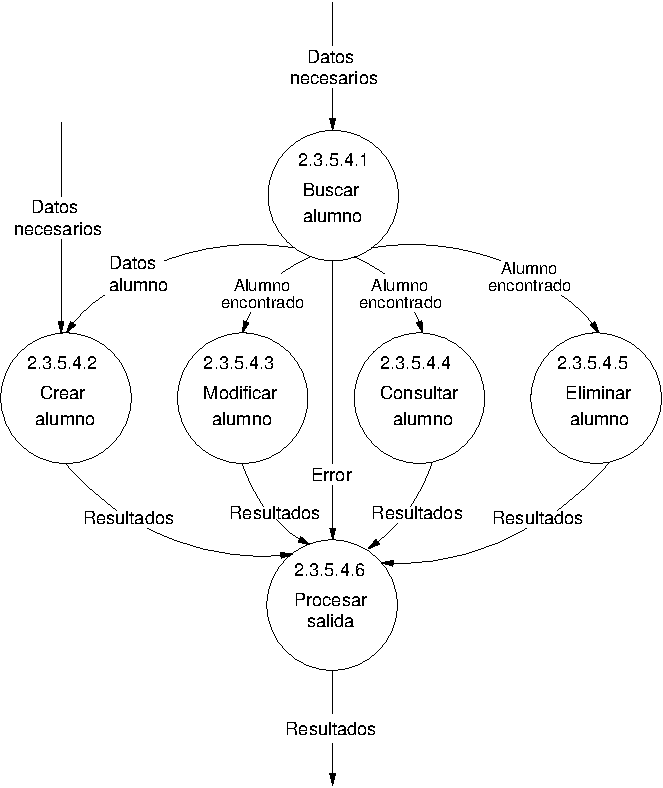
\includegraphics[]{08.Analisis_Funcional/8.2.DFDs/Niveles/Nivel5/AdministradorPrincipal/AdministrarUsuarios/AdministrarAlumnos/Diagramas/nivel5-AdministrarAlumnos.pdf}
      \caption{Nivel de abstracción 5: Administrar Alumnos (módulo
      Administrador principal).}
      \label{diagramaNivel5-AdministrarAlumnos}
    \end{center}
  \end{figure}
